\chapter{Verification of models in LAMMPS}
In this chapter, i verify that my LAMMPS setup reproduces known results from the literature. This is necessary to trust the model to go further with modifications. 
\section{TIP4P/ICE}
\section{United atom methane}
\section{Stabilizing methane hydrates}
The TIP4P/ICE potential should be able to stabilize a methane hydrate stucture. Therefore, I prepared an S1 hydrate using positions from \cite{Takeuchi2013}. These positions were derived using the TIP4P potential, so this configuration is not expected to be an equilibrium configuration for TIP4P/ICE. The hydrate equilibrated nicely, using a Nosé-Hoover $NPT$ thermostat with a temperature rising from $0$ to \SI{30}{\kelvin}. 

\begin{figure}
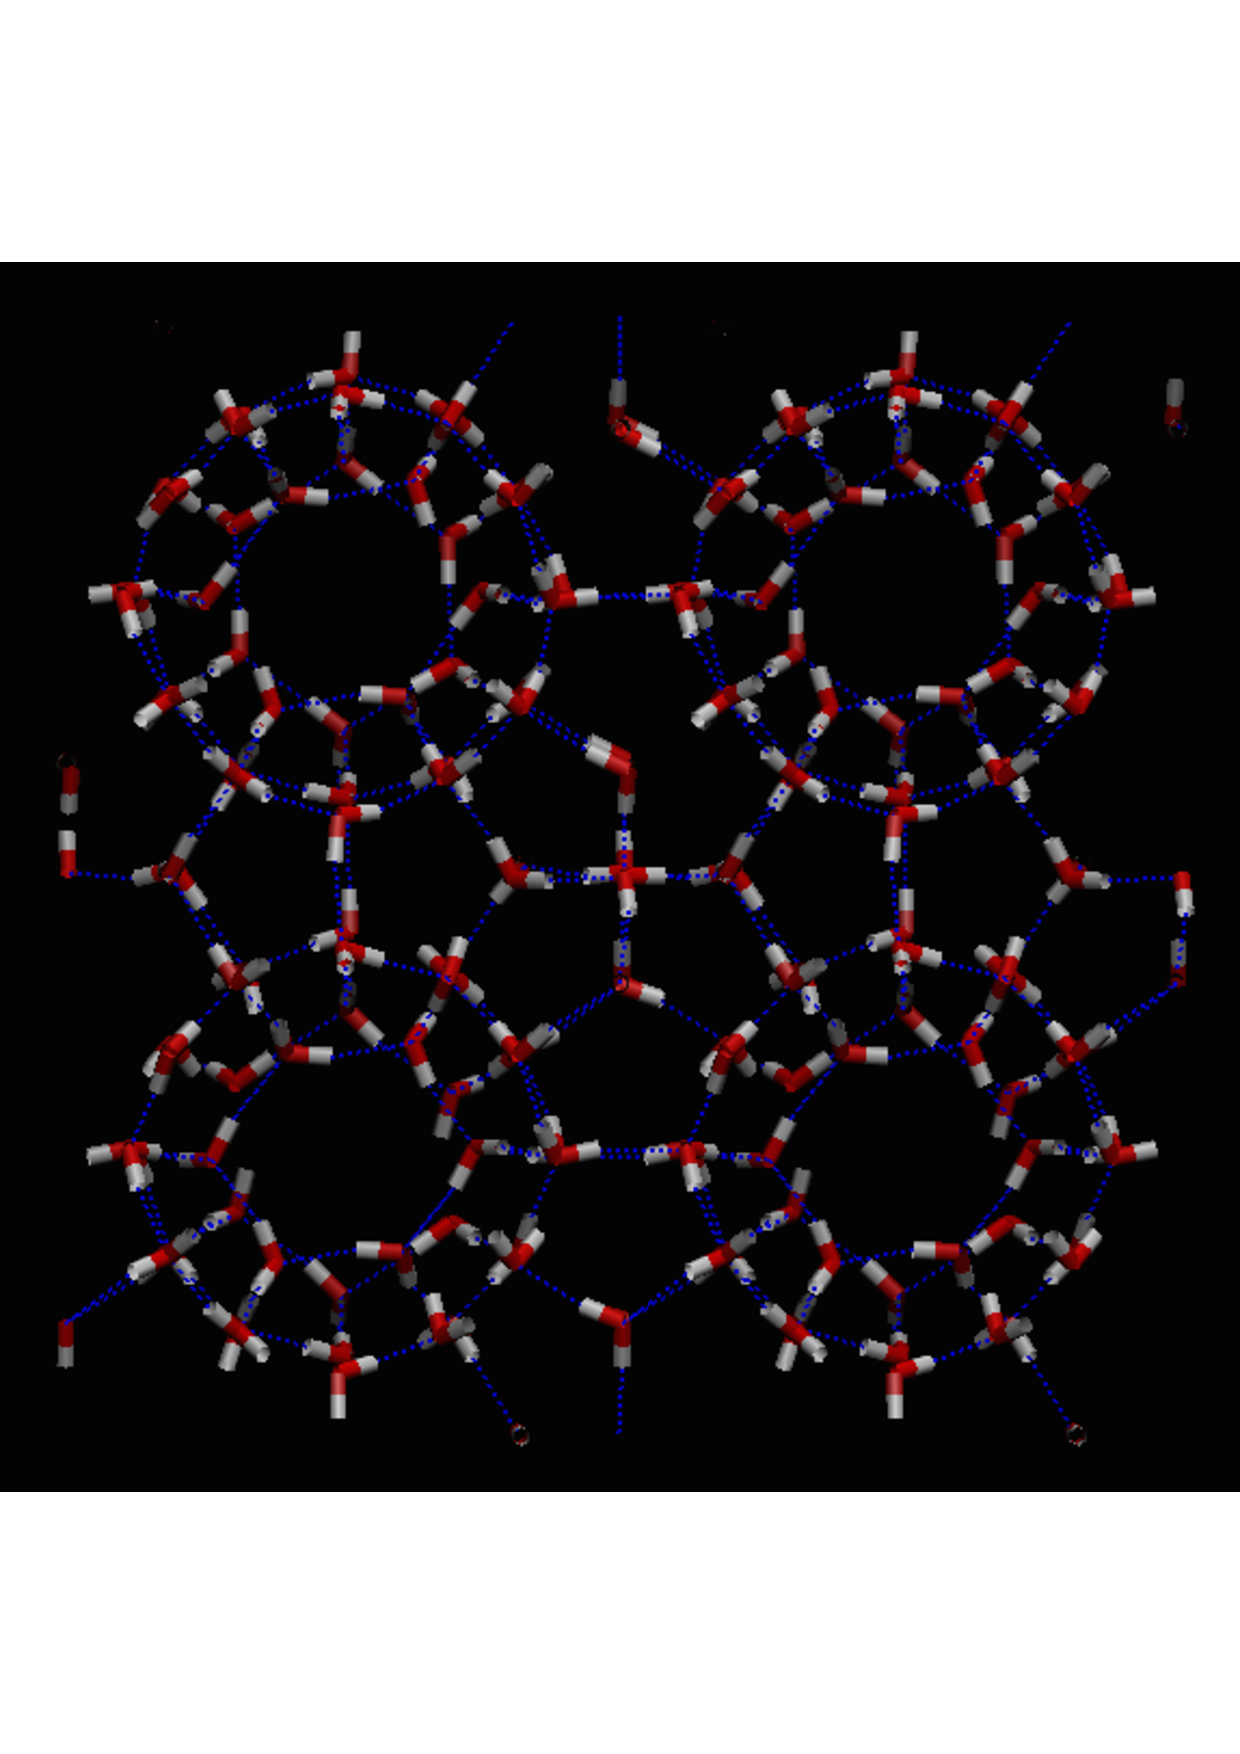
\includegraphics[width=\textwidth]{../snapshots/first_stable_hydrate.pdf}
\caption{Methane hydrate at low temperature. Rendered with VMD}
\label{fig:part2:first_hydrate}
\end{figure}

\section{Three-phase equilibrium line for methane hydrate}
Three-phase equilibrium simulations have been performed to check whether the model system is in the same ballpark as systems from the literature. Simulations have been performed on a system similar to the one in \cite{Conde2010}.

\section{Nucleation of methane hydrates?}
Nucleation of methane hydrates in a solution of water and methane is a rare event, and microsectond-simulations are required. 
